\section{Durchführung}
\label{sec:Durchführung}
\subsection{Untersuchung der Ablenkung des Elektronenstrahls im elektrischen Feld}
\label{subsec:ablenkung1}
Die Kathodenstrahlröhre wird gemäß den Abbilungen \ref{fig:kathode} und \ref{fig:schaltung1} beschaltet.

\begin{figure}[H]
  \centering
  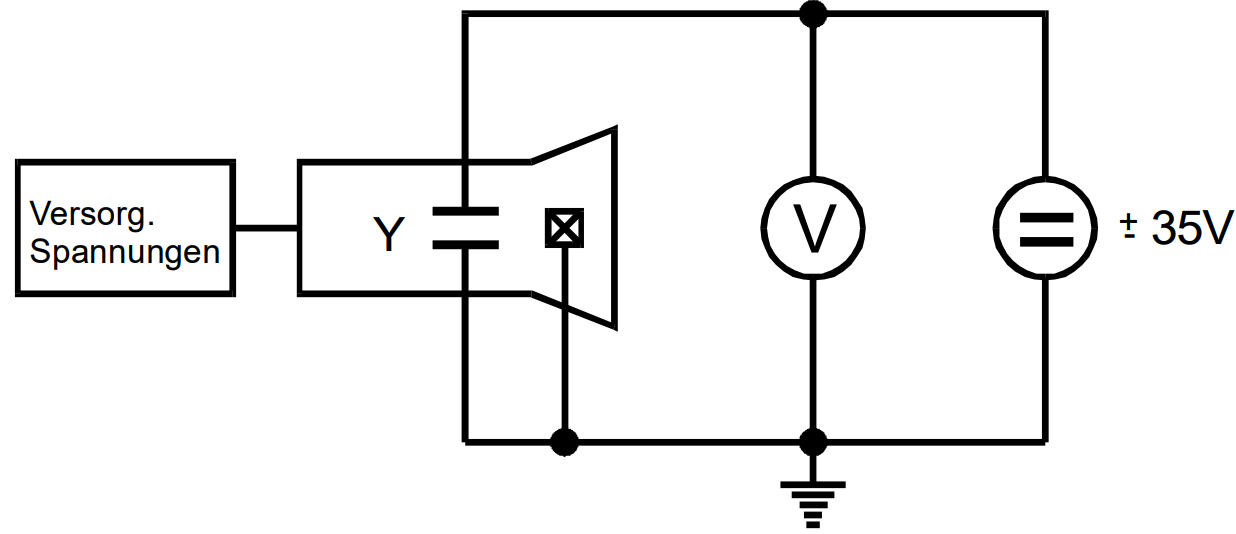
\includegraphics[width=250pt]{data/schaltung1.png}
  \caption{Skizze der Schaltung zur Messung der Ablenkung in Abhängigkeit der Ablenkspannung \cite{Versuchsanleitung501}.}
  \label{fig:schaltung1}
\end{figure}

Dabei bezeichnet
$U_\text{G}$ die Heizspannung. Die Ablenkplatten der Kathodenstrahlröhre werden
geerdet und an eine Spannungsquelle angeschlossen. Die am Wehnelt-Zylinder und
an den Fokussierungselektroden anliegenden Spannungen werden so eingestellt, dass
ein lokalisierter leuchtender Punkt auf dem Leuchtschirm zu sehen ist. Es wird eine
konstante Beschleunigungsspannung im Bereich von $\SI{180}{\volt}$ bis $\SI{500}{\volt}$
eingestellt. Die Spannung für die $x$-Ablenkung wird so eingestellt, dass der Leuchtpunkt
stets auf der $y$-Achse ist. Dann wird die Spannung für die vertikale Ablenkung nacheinander so
variiert, dass der Leuchtpunkt auf die neun jeweils äquidistant $\SI{6}{\milli\meter}$
voneinander entfernten Koordinatenlinien fällt. Die Messpaare der nötigen Ablenkspannung
und der Ablenkung werden notiert. Es werden insgesamt Messreihen für fünf verschiedene
Beschleunigungspannungen aufgenommen.

\subsection{Untersuchung einer Wechselspannung durch einen Kathodenstrahl-Oszillosgraphen}
\label{subsec:oszi}

Die Schaltung zur Untersuchung einer sinusförmigen Wechselspannung mithilfe der
Ablenkung eines Elektronenstrahls in einer Kathodenstrahlröhre ist in \ref{fig:schaltung2}
dargestellt.

\begin{figure}[H]
  \centering
  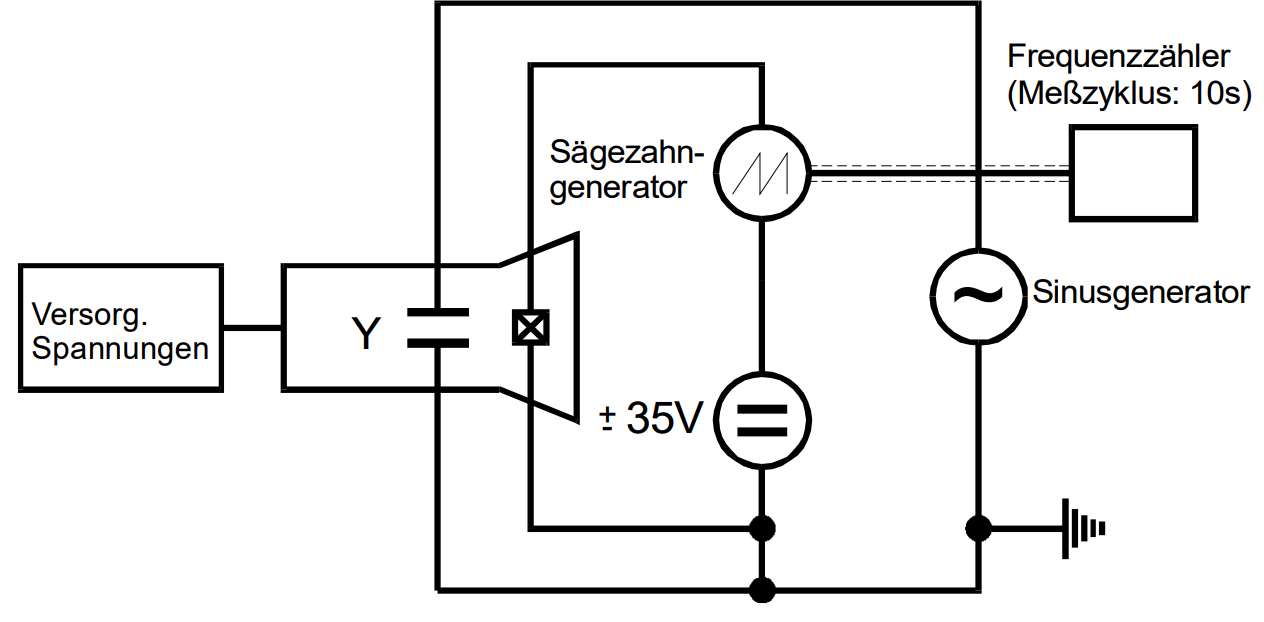
\includegraphics[width=250pt]{data/schaltung2.png}
  \caption{Skizze der Schaltung zur Bestimmung der Frequenz einer Wechselspannung \cite{Versuchsanleitung501}.}
  \label{fig:schaltung2}
\end{figure}

Dazu wird an die horizontale Ablenkung die Sägezahnspannung angelegt, die zu untersuchende
Sinusspannung wird an die vertikale Ablenkung angeschlossen.
Die Frequenz der Sägezahnspannung wird variiert, um für das Verhältnis von $f_\text{Si}$
und $f_\text{Sä}$ die Fälle $1/2 , \, 1, \, 2, \, 3$ zu realisieren.
Dies ist genau dann erreicht, wenn ein näherungsweise stehendes Bild auf dem Leuchtschirm
zu sehen ist. Das Verhältnis ist dann an der Anzahl der Wellen zu erkennen. Die eingestellte Frequenz
wird dann stets am Frequenzzähler abgelesen und notiert.

\subsection{Untersuchung der Ablenkung eines Elektronstrahls durch ein transversales Magnetfeld}
\label{subsec:daspraktikumistscheisse}
Die Kathodenstrahlröhre wird nun in die Mitte zwischen die Spulen eines Helmholtzspulenpaars
gestellt. Dieses wird so ausgerichtet, dass die Feldrichtung des Helmholtzfeldes
senkrecht zur Achse der Kathodenstrahlröhre steht und das Magnetfeld der Erde parallel
zur Achse der Röhre steht. Die Richtung des Erdmagnetfelds wird dabei durch ein Deklinatorium-Inklinatorium
festgestellt. Dadurch ist sichergestellt, dass der Elektronenstrahl in diesem Teil
des Versuchs vom Erdmagnetfeld unbeeinflusst bleibt. Die Kathodenstrahlröhre wird wie
zuvor beschaltet. Die Fokussierungsspannungen werden so angepasst, dass ein möglichst kleiner
Leuchtfleck auf dem Schirm zu sehen ist. Durch Anpassen der Ablenkspannungen wird
der Leuchtfleck auf die oberste Linie des Koordinatengitters des Schirms gelenkt.
Bei maximaler Spannung an dem Helmholtzspulenpaar wird nun die Stromstärke erhöht,
bis der Leuchtfleck zentriert auf der zweitobersten Linie liegt. Dieser Wert wird notiert.
So wird mit allen Linien verfahren, bis der Leuchtfleck an der untersten Linie ist.
Es werden zwei Messreihen für Beschleunigungspannungen von jeweils $\SI{250}{\volt}$ und
$\SI{400}{\volt}$ aufgenommen.
\subsection{Aufnahme eines Messwerts zur Bestimmung des Erdmagnetfelds}
\label{subsec:brauchtniemand}
Die Beschleunigungsspannung der Kathodenstrahlröhre wird möglichst niedrig geregelt.
Die Apparatur wrd parallel zu den Feldlinien des Erdmagnetfeldes ausgerichtet, sodass
keine magnetische Kraft auf den Elektronenstrahl wirkt. Der Leuchtpunkt wird durch
Einstellung der Ablenkspannungen in den Ursprung des Leuchtschirms verschoben.
Daraufhin wird die Apparatur in möglichst genaue Ost-West-Richtung gedreht, sodass
das Erdmagnetfeld senkrecht zum Elektronenstrahl steht und die magnetische Kraft maximal
ist. Aus diesem Grund verschiebt sich der Leuchtfleck auf dem Schirm signifikant.
Daraufhin wird der Strom $I$, der das Helmholtzspulenpaar durchfließt, so geregelt, dass
das Helmholtzfeld die magnetische Kraft des Erdmagnetfelds ausgleicht und den Leuchtfleck
zurück in den Ursprung ablenkt. Dieser eingestellte Strom wird notiert. In dem Fall
sind ist das Helmholtzfeld entgegengerichtet gleich zur Horizontalkomponente des Erd-
magnetfeldes.
\\
Zur Bestimmung der totalen Intensität des Erdmagnetfeldes muss der Inklinationswinkel
$\varphi$ bestimmt werden. Dies ist der Winkel des Erdmagnetfelds zur Horizontalen.
Dazu wird das Deklinatorium-Inklinatorium verwendet, das mithilfe einer magnetisierten
Nadel die Messung dieses Inklinationswinkels ermöglicht.
